\documentclass[acmsmall,review,authorversion]{acmart}
\usepackage{multirow}

\graphicspath{images}

\acmDOI{}
\acmJournal{FACMP}
\acmVolume{CSCI 5535}
\acmNumber{Spring 2020}

\usepackage[utf8]{inputenc}
\usepackage{minted}
\usepackage{listings}
\usepackage{hyperref}

\title{Boilerplate logger}
\subtitle{A logger for developers by developers}
\author{Evan Lee}
\affiliation{%
    \institution{University of Colorado Boulder}
    \city{Boulder}
    \state{Colorado}
}
\email{evan.n.lee@colorado.edu}
\date{May 2020}

\keywords{logging, boilerplate}

\setcopyright{rightsretained}
\acmYear{2020}
\copyrightyear{2020}


\newcommand{\code}[1]{\lstinline[basicstyle=\ttfamily\small]~#1~}

\begin{document}

\begin{abstract}
    The logging aspect of any software project always incurs a non-zero developer investment, both from a development and testing perspective as well as a operational and error tracing perspective. A significant portion of the thought and energy behind logging decisions arise from nearly-universal problems and use cases and yet still require each distinct developer to undergo the same rote process of decision making. Even with these factors and costs in play, logging is typically not considered as a first-class issue which leads to hidden cost in terms of development cycles or unnecessary iteration to assist in tracing and debugging. After having identified a widely realized use case of logging in dev-test cycles, we introduced and defined the concept of ``boilerplate logging'' and developed a Python logging library that largely abstracts the human component to logging decisions, simultaneously solving the hidden up-front development cost in logging decision making as well as eliminating any future costs in iterating on reactive postmortem logging.
\end{abstract}

\maketitle

\section{Introduction}

    % What is the problem?
    Logging as a language construct is a double-edged sword; developers want all the information they can get for use in troubleshooting, debugging, and development, but this often comes as a latent cost in terms of either lines of code or in logical paths designed specifically to handle development logging use cases. This causes a balancing act: certainly early into the development cycle, logging statements are vastly prevalent in code and the statements themselves are used to great effect on a regular basis. However, this pattern shifts as code becomes more mature. Production processes almost certainly deactivate nearly all of the logs put in place for development and leave lines of code orphaned and without use. In some situations -- for the sake of performance or cleanliness -- additional iteration is performed with the sole purpose of removing log lines that are no longer needed. This balancing act can be represented as a spectrum: from one side being extremely verbose logs to the other side being total lack of logs and only application code.

    % Why is this problem important?
    All of this activity is largely universal in the development world and leads to countless development cycles and engineering hours hidden away from the bottom line. In addition, some cases present themselves where application logic is even warped or influenced by the presence of logging which should be considered a second-class citizen when compared to core functionality and logic; take an example where code must be written to decide what a log message should itself say or be formatted as.

    % Why is the problem hard?
    To reiterate: the cost of managing this balancing act is hidden at best and outright obscured at worst. Developers even considering changes that have to do with logging incur a small, nearly insignificant cost. These small costs add up over the span of the industry and especially over the span of time. In addition, logging at its heart is a subjective activity. Different developers from different backgrounds using different languages with different frameworks all will use unique styles of logging and make unique decisions on log positions, formatting, substance, and level. This presents difficulty in the qualitative analysis of logging and generally throws a wrench into any standardization activity.

    % What is our contribution?
    Our contribution to this effort is two-fold: a collection and analysis of log usage in widely-used open-source libraries as well as an implementation that displays the ideas and positions presented below. Popular open-source libraries and tools are of particular interest in this space as not only do they have a wide range of contributors, but there is a communal sense of ``being a good neighbor'' when writing open-source code; particular care is given to the logging statements that are eventually committed and merged into the mainstream base and thus particular thought and effort is given to the balancing act between verbosity and utility.

\section{Overview}

    In order to assist the reader in visualizing the analysis and ideas that this paper presents as well as the benefits of implementation, we will cover a code example from a widely-used Python library for interacting with SOAP interfaces: \code{python-zeep}. The code snippet can be found in Listing \ref{lst:explosion-example}\footnote{Source: \href{https://github.com/mvantellingen/python-zeep/blob/4df383021e31372c111bc26cbf2e4535deaee04e/src/zeep/transports.py\#L47}{python-zeep/transports.py}, lines 47-84. (sha: 4df383021e31372c111bc26cbf2e4535deaee04e)}. Reading through this 31-line snippet, most of the lines written by the developer deal with logging in one way or another, whether that is making logging decisions (lines 2-5, 12-22) or dealing with emitting log messages themselves (lines 6, 24). In fact, only three lines (lines 8-10) deal with any actual functionality that this method is meant to drive.

    One of the explicit goals of boilerplate logging is to provide key information to developers at significant breakpoints in code. The log messages in lines 6 and 24 are concerned mainly with two channels of boilerplate log statements -- line 6 provide a message for the inputs of the example method and line 24 provides a message for the output of the example method. So while the format of the logging output may differ from Snippet \ref{lst:explosion-example} to Snippet \ref{lst:cleaned-example}, the code can be refactored to instead use boilerplate logging to accomplish the same goals by activating the required channels within the boilerplate logger itself.

    Take the output of the log message as-written on line 6:

    \begin{quote}
    \code{HTTP Post to https://api.colorado.edu/: \{"test": "test"\}}
    \end{quote}

    and take the output of a boilerplate logger log message that would be emitted upon the invocation of the \lstinline{post} method:

    \begin{quote}
        \code{[transports.post]: [args: ('https...', \{"test": "test"\}, \{\})] [kwargs: \{\}]}
    \end{quote}

    The formatting of the messages differ, but the same set of information is imparted to the reader.

    In addition, consider the additional benefit that boilerplate logging provides in the above example. Take a situation where a future maintainer of the code must also capture the \lstinline{header} object being provided to the \lstinline{post} method in the logs for any reason -- now an additional iteration of code must be developed and committed.

    \begin{listing}[H]
    \begin{minted}[
        mathescape,
        numbersep=5pt,
        frame=lines,
        framesep=2mm,
        linenos
    ]{python}
    def post(self, address, message, headers):
        if self.logger.isEnabledFor(logging.DEBUG):
            log_message = message
            if isinstance(log_message, bytes):
                log_message = log_message.decode("utf-8")
            self.logger.debug("HTTP Post to %s:\n%s", address, log_message)

        response = self.session.post(
            address, data=message, headers=headers, timeout=self.operation_timeout
        )

        if self.logger.isEnabledFor(logging.DEBUG):
            media_type = get_media_type(
                response.headers.get("Content-Type", "text/xml")
            )

            if media_type == "multipart/related":
                log_message = response.content
            else:
                log_message = response.content
                if isinstance(log_message, bytes):
                    log_message = log_message.decode(response.encoding or "utf-8")

            self.logger.debug(
                "HTTP Response from %s (status: %d):\n%s",
                address,
                response.status_code,
                log_message,
            )

        return response
    \end{minted}
    \caption{An example of code explosion due to boilerplate logging.}
    \label{lst:explosion-example}
    \end{listing}

    \begin{listing}[H]
    \begin{minted}[
        mathescape,
        numbersep=5pt,
        frame=lines,
        framesep=2mm,
        linenos
    ]{python}
    import boilerplate as bp

    """
    Not passing anything or passing "all" is the same as:
    @bp.log("inputs")
    @bp.log("outputs")
    """

    @bp.log
    def post(self, address, message, headers):
        response = self.session.post(
            address, data=message, headers=headers, timeout=self.operation_timeout
        )
        return response
    \end{minted}
    \caption{The same code as Listing \ref{lst:explosion-example}, but using the boilerplate logger.}
    \label{lst:cleaned-example}
    \end{listing}

    \subsection{Distinctions}

    The key distinction between boilerplate logging and that of other standard logging libraries is a matter of control. In general, standard third-party and language-specific logging libraries advertise themselves as offering a great degree of fine-grained control in terms of logging output, formats, and location. We take the stance that in many cases identified as ``boilerplate'', offering control to this degree actually is a long-term detriment. Boilerplate logging aims to move decision-making out to more coarse-grained controls to eliminate overhead that comes with subjective decision making with respect to logging outputs and formatting.

    Specifically, boilerplate logging is meant to be a to be a complement to application-specific logging, not a replacement. Our initial iteration of a boilerplate logging library written in Python actually leverages use of the standard Python logging library in its internal workings. The goal of boilerplate logging is remove the overhead around certain boilerplate log use cases. This allows developers to focus logging efforts on application-specific logging.

    \subsection{Contributions}

    The contributions of this paper include:

    \begin{itemize}
        \item The definition and boundaries of boilerplate logging, specifically as a sub-category of logging use cases.
        \item Data and analysis of open and closed source projects implemented in Python and the characterization of logging statements within.
        \item An implementation of the idea presented in a Python 3+ logging library.
    \end{itemize}

\section{Research \& Analysis}

We gathered both qualitative and quantitative data with respect to logging patterns and use cases, performing analysis to uncover the niche that our identified ``boilerplate logging'' fit into over the course of software development. For our quantitative data, we performed code analysis over a set of open and closed source software projects. For our qualitative data, we conducted a survey targeted at professional software developers on personal use of logging patterns and software background.

\subsection{Data}

\subsubsection{Quantitative Metrics}

We built a data set by analyzing various open and closed source projects of different purposes and categorizing the nature of logging statements within source code.

The criteria we used in selecting open source projects for analysis were:

\begin{itemize}
    \item actively developed and maintained by the community at large; latest commit or pull request within the last 90 days.
    \item extensively used in other projects; a GitHub ``used by'' metric of at least 1000.
    \item a premiere library in the target functionality of choice (widely recommended as the library of choice for that particular use case); present on the Awesome Python list \cite{awesome-python}.
    \item made use internally of logging; either built-in Python \code{logging} or other third-party logging library.
\end{itemize}

For those open-source projects that we identified made some use of logging internally and for the closed source projects we had access to, we collected the following metrics for analysis:

\begin{itemize}
    \item lines of code per file (ignoring whitespace and comments)
    \item logging lines of code per file (emitting logs or dealing with log messages, formatting, decisions, etc)
    \item boilerplate logging lines of code per file (logging lines and supporting lines that were identified to deal with boilerplate logs)
    \item maximal gain ratio (<total lines of code - boilerplate lines>/<total lines>)
\end{itemize}

These metrics deal with one area of development cost that we view as "unnecessary iteration" and are measurable and concrete.

The raw, low level results are available for inspection as requested. Table \ref{tab:agg-data} on page \pageref{tab:agg-data} is an an aggregated summary of our collected findings.

\begin{table}[h]
\centering
\begin{tabular}{|r|c|c|}
\hline
\textbf{source code status}                  & \textbf{open}               & \textbf{closed}            \\ \hline
\textbf{\# of files}                         & 812                         & 141                        \\ \hline
\textbf{\# of lines}                         & 115804                      & 21621                      \\ \hline
\textbf{average lines per file}              & 142.62                      & 153.34                     \\ \hline
\textbf{average logging lines per file}      & 0.39                        & 5.57                       \\ \hline
\textbf{average boilerplate lines per file}  & 0.06                        & 1.87                       \\ \hline
\textbf{log lines (\% of total)}             & 0.28\%                      & 3.70\%                   \\ \hline
\textbf{boilerplate lines (\% of log lines)} & 1.63\%                      & 21.88\%                    \\ \hline
\textbf{boilerplate lines (\% of total)}     & 0.04\%                      & 1.17\%                     \\ \hline
\end{tabular}
\caption{Aggregated statistics over analyzed source code files.}
\label{tab:agg-data}
\end{table}

\subsubsection{Qualitative Metrics}

A second area of development cost we identify as ``development time/development cycles wasted''. We were unable to measure and analyze this cost quantitatively, so we took a qualitative approach. We polled a number of software developers from different backgrounds on their logging usage patterns. Specifically, the questions that we asked were:

\begin{itemize}
    \item What language do you primarily develop in?
    \item Would you consider yourself a front-end or back-end developer?
    \item During development of a \textbf{new} feature, what percentage of work would you say deals in one way or another with boilerplate logging?
    \item During development or iteration on a \textbf{previously-existing} feature or code base, what percentage of work would you say deals in one way or another with boilerplate logging?
\end{itemize}

Twenty-nine respondents answered the survey we sent out to professional engineers and colleagues in the industry.

\begin{figure}[h]
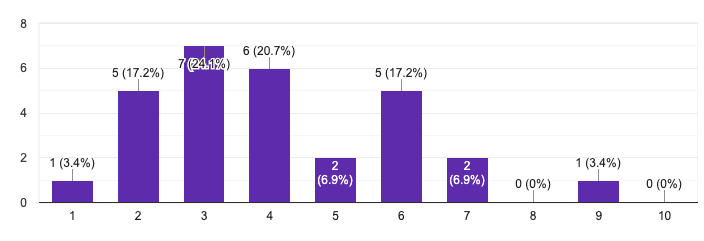
\includegraphics[width=\linewidth]{images/bp_survey_time_new.png}
\caption{Responses to: ``During development of a \textbf{new} feature, what percentage of work would you say deals in one way or another with boilerplate logging?''. X-Axis represents percentage of work (take value times 10\%), Y-Axis represents number of responses.}
\label{fig:new}
\centering
\end{figure}

\begin{figure}[h]
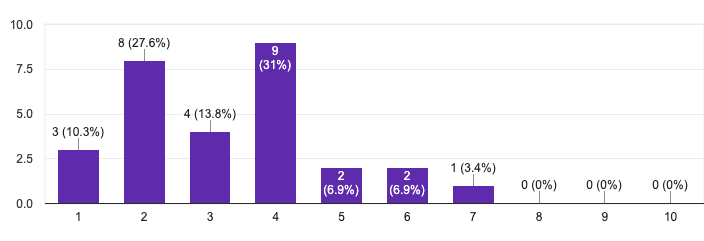
\includegraphics[width=\linewidth]{images/bp_survey_time_prev.png}
\caption{Responses to: ``During development or iteration on a \textbf{previously-existing} feature or code base, what percentage of work would you say deals in one way or another with boilerplate logging?''.}
\label{fig:prev}
\centering
\end{figure}

\subsection{Conclusions}

From the quantitative data gathered, we discovered a pattern in open source software that we conjecture is due to the ``good citizen'' nature of open source projects: most log functionality is entirely disabled or provided via hooks and left as an exercise to the caller. In fact, many open source projects perform some form of linting and explicitly require that logging statements that are considered to be boilerplate be left out of pull requests into the main branch. This fact correlates with our view that boilerplate logging is primarily a development activity and generally is not considered suitable for production usages. This also reinforced our understanding that boilerplate logging was in use, but the cost was felt twofold: once in the developer writing code that contains boilerplate logging statements for use in the course of development, and the second time in that developer needing to ``clean up'' the boilerplate logs for use in production.

These conclusions and understandings were also reinforced by the qualitative data gathered. Even with the color that the data we gathered via survey is subjective, we conclude that effort expended into boilerplate logging during development is not insignificant. The majority of developer responses range from 20-40\% of work spent on boilerplate logging activities. Given our findings with respect to downstream statistics like proportion of boilerplate lines in total (Table \ref{tab:agg-data}), these statistics support our assertions that boilerplate logging is a largely ``hidden'' cost that incurs repeated cost in terms of development cycles and at each iteration.

\section{Implementation}

To display our ideas around the concept of boilerplate logging, we implemented a simple logging library in Python, aptly named \code{boilerplate}. Our initial iteration of the \code{boilerplate} library includes functionality to abstract two identified ``boilerplate'' use cases: (a) inputs and outputs to a function or method and (b) a exception ``trace'' logger that caches the inputs and outputs of N calls (configurable) leading up to a thrown exception to provide more information than a typical stacktrace. Included with the implementation is an example Python script showing the features provided by our \code{boilerplate} library.

\subsection{Inputs \& Outputs}

The main entry point to our implemented logging library is as function and method decorators\footnote{See: \href{https://www.python.org/dev/peps/pep-0318/}{https://www.python.org/dev/peps/pep-0318/}} that developers can use to annotate the calls that they wish to have boilerplate logged, without any additional code required. The library uses these annotations to decide which function invocations to log as well as which channels to log. There are currently only two channel definitions: ``inputs'' and ``outputs'', and not specifying a specific channel will activate both channels by default. See Listing \ref{lst:invocation} for examples of how to trigger the boilerplate logger.

\begin{listing}[H]
    \begin{minted}[mathescape, numbersep=5pt, frame=lines, framesep=2mm, linenos]{python}
import boilerplate as bp

@bp.log
def add(x, y):
    return x + y

@bp.log("inputs")
def subtract(x, y):
    return x - y

@bp.log("outputs")
def multiply(x, y):
    return x * y

add(1, 1)
subtract(2, 1)
multiply(4, 5)
    \end{minted}
    \caption{Invocation examples of the boilerplate logger.}
    \label{lst:invocation}
\end{listing}

Under the hood, these decorators wrap the annotated calls with code hooks into the boilerplate library, which makes decisions on what to log and with what format. Our boilerplate library leverages the use of the Python standard \code{logging} library and exposes a lower-level \code{logger} object that has the same API as a built-in Python \code{logger} object which is accessible via \code{boilerplate.logger} or via \code{logging.getLogger("boilerplate")}. This provides a level of customization and familiarity that the built-in Python logging library exposes, including configurations like where to log (standard out, to a file handler, etc) and what the log format should be, although the messages themselves are of a standard format.

\begin{listing}[H]
    \begin{minted}[mathescape, numbersep=5pt, frame=lines, framesep=2mm, linenos]{bash}
[__main__.add] inputs: [args: (1, 1)] [kwargs: {}]
[__main__.add] returns: [2]
[__main__.subtract] inputs: [args: (2, 1)] [kwargs: {}]
[__main__.multiply] returns: [20]
    \end{minted}
    \caption{Logging output of the boilerplate logging library, of the code from Listing \ref{lst:invocation}.}
    \label{lst:log-examples}
\end{listing}

Since our library makes use of the Python standard logging library and is namespaced with the name \code{"boilerplate"}, developers can mix and match their application-specific logs in with the boilerplate logs or direct them to different locations. For example, a developer may find it useful to incorporate the boilerplate logs into their own specific applications on disk or in an external data store. To reduce the amount of noise, the boilerplate logger can also be disabled via standard Python logging libraries API without any change in code.

\subsection{Tracing}

Typical stack traces are often noisy and provide trace-backs that simultaneously contain too much and not enough information. Java developers in particular often have to deal with large, noisy stack traces that contain system or base language calls and provide no pertinent information to the developer besides being able to trace where exactly an exception occurred in terms of line number and column number. Oftentimes this information is not even sufficient to help the developer track down the issue. Development cycles are then wasted in placing debug logging statements at certain points along the execution path in order to provide a view into the changing state of a program.

Our logging library implements a feature that allows developers to register functions that may be in the critical path of an error or exception occurring. This functionality is unique in that the logs themselves are not emitted unless an exception occurs in one of the registered functions or there is an explicit call to flush the logs and emit them to the target location. This method of tracing and emitting keeps logs clean and provides more relevant, less noisy error analysis tools to developers in the course of development.

This registration action is exposed by our library again as a function decorator, with the syntax being \code{@boilerplate.trace}. Trace logs have both ``inputs'' and ``outputs'' channels activated for all annotated calls. Log statements are pushed to an in-memory buffer and trimmed to a configurable length in order to only keep the most relevant calls leading up to the exception.

Upon the trigger of an unhandled exception occurring or on a manual trigger by the developer in code, the logs in memory are flushed using the Python standard logging library to wherever the target location is (configurable, standard out by default).

\begin{listing}[H]
    \begin{minted}[mathescape, numbersep=5pt, frame=lines, framesep=2mm, linenos]{python}
import boilerplate as bp

@bp.trace
def add(x, y):
    return x + y

@bp.trace
def subtract(x, y):
    return x - y


@bp.trace
def multiply(x, y):
    return x * y

add(1, 1)
subtract(2, 1)
bp.flush()

bp.register_uncaught_exception_handler()
multiply(4, 5)
raise Exception("trigger flush of boilerplate logs")
    \end{minted}
    \caption{Trace examples of the boilerplate trace logger.}
    \label{lst:trace-invocation}
\end{listing}


\begin{listing}[H]
    \begin{minted}[mathescape, numbersep=5pt, frame=lines, framesep=2mm, linenos]{bash}
== BOILERPLATE TRACE:
[__main__.add] inputs: [args: (1, 1)] [kwargs: {}]
[__main__.add] returns: [2]
[__main__.subtract] inputs: [args: (2, 1)] [kwargs: {}]
[__main__.subtract] returns: [1]
== END BOILERPLATE TRACE ==
Registered as uncaught exception handler!
Exception occurred; flushing boilerplate trace.
== BOILERPLATE TRACE:
[__main__.multiply] inputs: [args: (4, 5)] [kwargs: {}]
[__main__.multiply] returns: [20]
== END BOILERPLATE TRACE ==
Traceback (most recent call last):
  File "trace_example.py", line 25, in <module>
    raise Exception("trigger flush of boilerplate logs")
Exception: trigger flush of boilerplate logs
    \end{minted}
    \caption{Trace logging output of the boilerplate logging library, of the code from Listing \ref{lst:trace-invocation}.}
    \label{lst:trace-log-examples}
\end{listing}


\section{Evaluation}

We subscribed to two measures of success, each of which relates to the sectors of cost associated with boilerplate logging. The first is logical lines of code or LLOC, which tracks the cost associated with needing to write lines of code to support boilerplate use cases. The second is the maintainability index or the maintainability score, which is expanded upon below. The maintainability index tracks the cost associated with future support and iteration on a code base by future developers.

In order to measure the impact of our success, we developed two code bases -- the control iteration does not use our boilerplate logging library and the test iteration is the same code base, but manually refactored to use our boilerplate logging library.

We made use of the tool Radon \cite{radon}, which provides the four syntactic program metrics we are interested in:

\begin{itemize}
    \item lines of code (logical, source, comments, etc)
    \item cyclomatic complexity  \cite{wiki:mccabe} (AKA McCabe complexity; number of logical decisions)
    \item maintainability index (ease of long-term support and change; supported by Microsoft Visual Studio)
    \item various Halstead metrics \cite{wiki:halstead} (difficulty, effort, time to program, expected bugs, etc)
\end{itemize}

When compared to our control iteration, the success thresholds for our test iteration are:

\begin{itemize}
    \item a \textbf{decrease} in lines of code
    \item an \textbf{increase} in maintainability
\end{itemize}

Some other metrics we would like to see changes in across iterations, but are not fully considered in terms of evaluation are:

\begin{itemize}
        \item a \textbf{decrease} in time required to program
    \item a \textbf{decrease} in cyclomatic complexity
    \item a \textbf{decrease} in expected bug count
\end{itemize}

We chose an inner utility module in a closed-source application that we believed had particular potential to improve through the use of boilerplate logging. This particular utility module served the rest of the application by holding the functionality for reaching out to external systems such as other devices or APIs to fetch data, and so held a lot of potential in having many particular entry and exit points for data.

We first used Radon to record the metrics of interest before we refactored the module to instead use our boilerplate logging library. We then used Radon to inspect the metrics after refactor. See Table \ref{tab:evaluation-metrics} for a summary of results.

For the metrics that were targeted explicitly, our \code{boilerplate} logging library succeeded with an across the board improvement in both logical lines of code and maintainability index. Of particular interest were the other complexity and syntactic measure metrics that \code{boilerplate} could not move the needle significantly in this particular example. The time required, McCabe complexity, and expected bugs did not change in any significant capacity. We conjecture this is due to the nature of the example chosen, where the code did not include any logical code decisions with regards to logging. Take our original example from \code{python-zeep}, \code{transports.py} where the original average McCabe complexity is \textbf{3.125} and the post-refactor McCabe complexity is \textbf{2.25} (-38.89\%). We consider this example a best-case display of the performance of our \code{boilerplate} library.

\begin{table}[h]
\centering
\begin{tabular}{|r|r|c|c|c|c|c|}
\hline
 &  & \textbf{File 1} & \textbf{2} & \textbf{3} & \textbf{4} & \textbf{5} \\ \hline
\multirow{3}{*}{\textbf{logical lines of code}} & original & 44 & 308 & 97 & 64 & 255 \\ \cline{2-7}
 & refactored & 43 & 295 & 84 & 63 & 249 \\ \cline{2-7}
 & change & -2.27\% & -4.22\% & -13.4\% & -1.56\% & -2.35\% \\ \hline
\multirow{3}{*}{\textbf{maintainability score}} & original & 77.65 & 38.10 & 65.85 & 60.62 & 31.04 \\ \cline{2-7}
 & refactored & 78.30 & 38.94 & 67.75 & 61.75 & 31.41 \\ \cline{2-7}
 & change & +0.83\% & +2.16\% & +2.80\% & +1.83\% & +1.18\% \\ \hline
\multirow{3}{*}{\textbf{time required score}} & original & 0.645 & 484.207 & 41.743 & 31.523 & 524.023 \\ \cline{2-7}
 & refactored & 0.645 & 484.207 & 41.743 & 31.523 & 524.023 \\ \cline{2-7}
 & change & 0.0 & 0.0 & 0.0 & 0.0 & 0.0 \\ \hline
\multirow{3}{*}{\textbf{McCabe complexity}} & original & 2.2 & 5.056 & 6.5 & 4.5 & 5.0 \\ \cline{2-7}
 & refactored & 2.2 & 5.056 & 6.25 & 4.5 & 5.0 \\ \cline{2-7}
 & change & 0.0 & 0.0 & -0.25 & 0.0 & 0.0 \\ \hline
\multirow{3}{*}{\textbf{expected bug count}} & original & 0.003 & 0.354 & 0.066 & 0.061 & 0.490 \\ \cline{2-7}
 & refactored & 0.003 & 0.354 & 0.066 & 0.061 & 0.489 \\ \cline{2-7}
 & change & 0.0 & 0.0 & 0.0 & 0.0 & -0.001 \\ \hline
\end{tabular}
\caption{Radon syntactic metrics, original \& refactored.}
\label{tab:evaluation-metrics}
\end{table}

\section{Related Work}

    \subsection{Standarization.} The industry has made similar efforts in the area of standarization of logs, which really deals with the abstraction of the human element away and instead introduces a controlled process around software logging. Some ideas introduced are the concepts of log composition \cite{DBLP:conf/dls/Marron18} and enhancement \cite{DBLP:journals/tocs/YuanZPZS12}. However, this research deals explicitly with the idea of standardization through total abstraction, whereas similar efforts continue to leave an aspect of the human element in the practice of logging.

    \subsection{Decision making.} There is more interest in understanding the motivation and usage behind log statements. Other efforts include attempting to understand the justification behind the locations developers place logging statements \cite{DBLP:conf/icse/FuZHLDLZX14} and the quality and characteristics behind logging statements themselves \cite{DBLP:conf/icse/YuanPZ12}. This research takes a similar approach to perform its analysis but utilizes the insights gleaned in a more naïve context, preferring instead a more black-and-white, dumb approach to categorization or use case analysis.

\section{Conclusion}

This paper introduced and defined the concept of \underline{boilerplate logging} and iterated the use cases under the boilerplate umbrella. We explored the sectors of cost associated with boilerplate logging and performed qualitative and quantitative analysis on data gathered from existing code bases and responses to the survey we conducted to showcase our ideas in numbers and data. Out of the use cases explored, we developed a Python logging library aptly called \code{boilerplate} implemented to address two of the use cases identified as ``boilerplate''. Finally, we showed that leveraging the use of \code{boilerplate} has the potential to improve metrics such as logical lines of code, maintainability score, and McCabe complexity, providing another tool to increase efficiency of development across the industry.

\begin{acks}
I would like to thank Professor Evan Chang and Benno Stein for their teachings and feedback on iterations of this paper. I would also like to thank the friends and colleagues that responded to the survey and spent their time and effort to provide their data.
\end{acks}


\bibliographystyle{ACM-Reference-Format}
\bibliography{refs}


\end{document}
